\documentclass{article}
% to compile a preprint version, e.g., for submission to arXiv, add add the
% [preprint] option:
%     \usepackage[preprint]{neurips_2020}

% to compile a camera-ready version, add the [final] option, e.g.:
%     \usepackage[final]{neurips_2020}

% to avoid loading the natbib package, add option nonatbib:
     \usepackage[nonatbib]{neurips_2020}

\usepackage[utf8]{inputenc} % allow utf-8 input
\usepackage[T1]{fontenc}    % use 8-bit T1 fonts
\usepackage{hyperref}       % hyperlinks
\usepackage{url}            % simple URL typesetting
\usepackage{booktabs}       % professional-quality tables
\usepackage{amsfonts}       % blackboard math symbols
\usepackage{nicefrac}       % compact symbols for 1/2, etc.
\usepackage{microtype}      % microtypography
% \usepackage{titling}
\usepackage{enumitem}
\usepackage{hyperref}

\usepackage{listings}
\usepackage{xcolor}
\usepackage{graphicx}


\definecolor{codegreen}{rgb}{0,0.6,0}
\definecolor{codegray}{rgb}{0.5,0.5,0.5}
\definecolor{codepurple}{rgb}{0.58,0,0.82}
\definecolor{backcolour}{rgb}{0.95,0.95,0.92}

\lstdefinestyle{mystyle}{
    backgroundcolor=\color{backcolour},   
    commentstyle=\color{codegreen},
    keywordstyle=\color{magenta},
    numberstyle=\tiny\color{codegray},
    stringstyle=\color{codepurple},
    basicstyle=\ttfamily\footnotesize,
    breakatwhitespace=false,         
    breaklines=true,                 
    captionpos=b,                    
    keepspaces=true,                 
    numbers=left,                    
    numbersep=5pt,                  
    showspaces=false,                
    showstringspaces=false,
    showtabs=false,                  
    tabsize=2
}

\lstset{style=mystyle}



\title{Catastrophic Forgetting: An Extension of Current Approaches}
% \subtitle{Advised by Professor Julia Kempe and Artem Vysogorets}
% AT Note: Using NEURIPS 2020 format 
% \author{(Author)}
\begin{document}

\maketitle


\begin{abstract}
We present an alternative algorithmic approach to catastrophic forgetting. We extend Wortsman et al.'s (2020) work on continual learning, \emph{Supermasks in Superposition}, by appplying an alternative masking technique.


Code available at: 

\textbf{Keywords:} Catastrophic forgetting, Continual learning, Binary networks, Masking

\end{abstract}



\section{Introduction}
Catastrophic forgetting is an area of active research in the continual learning space. Catastrophic forgetting, the ability to learn multiple tasks sequentially without forgetting, was originally discussed in McCloskey and Cohen's (1989) paper \emph{The Sequential Learning Problem} as well as in Ratcliff's (1990) work \emph{Constraints Imposed by Learning and Forgetting Functions}. 

More recently, research done by Wortsman et al. propose the use of supermasks in superposition (SupSup), which is "capable of sequentially learning thousands of tasks without catastrophic forgetting." [Wortsman et al., 2020] Their SupSup model uses a "randomly initialized, fixed base network and for each task finds a subnetwork (supermask) that achieves good performance." [Wortsman et al., 2020] Their approach uses gradient-based optimization to find the best performing linear superpostion that minimizes output entropy. 

Our analysis attempts to extend this approach by specifying linear combinations of supermasks rather than using a randomly initialized set of masks. Particularly, our rationale for this algorithmic extension is to (1) explore the ways through which we can use deep learning architectures without over-parametrization, as well as to (2) identify additional ways through which we can maximize resources as more computations in edge computing and continual learning occur on off-server devices. 


\section{Background and Related Work}

For this analysis, we studied two main approaches to catastrophic forgetting; namely (1) pruning and (2) masking. Comparing these two approaches, we see that pruning increases model capacity by removing low impact weights, while masking achieves this capacity increase by applying filters to neurons. Additionally, pruning approaches keep the old weights related to each neuron layer for training during the latter stages, while the core models in masking approaches do not modify these weights. The order of the training matters in pruning approaches, while in masking approaches it does not matter. Interestingly, model accuracy tends to degrade as more tasks are added in pruning approaches, as compared to masking approaches. And lastly, model capacity is limited for pruning approaches, while model capacity is unlimited for masking approaches, although masking requires initial memory overhead.

For our particular extension, we decided to focus on masking approaches, specifically by applying linear combinations in addition to SupSup's approach to binary masks. 

\subsection{Catastrophic Forgetting}


\subsection{Continual Learning}
In their research \emph{Continual Learning via Neural Pruning} (CLNP), Golkar et al, (2019) introduce a new method in lifelong learning which uses "fixed capacity models based on neuronal model sparsification." [Golkar et al., 2019] Namely, CLNP trains subsequent tasks using inactive neurons and filters of their sparsified network, which thus causes no deterioration to the performance of previously seen tasks. 

Golkar et al.'s research also introduces the concept of graceful forgetting, which is the idea that "it is preferable to suffer a small amount of forgetting in a controlled manner if it helps regain network capacity and prevents uncontrolled loss of performance during the training of future tasks." [Golkar et al., 2019] They empirically show that the use of activation-based neural pruning sparsification schemes can significantly outperform other approaches that are based on "weight elasticity". 


\subsection{Supermasks in Superposition}
Wortsman et al. (2020) present the SupSup models which can be (1) trained entirely "without task identity information" and (2) stored in a "constant-sized reservoir by implicitly storing them as attractors in a fixed-sized Hopfield network." [Wortsman et al., 2020] In their paper, they discuss different scenarios that show how a SupSup model can learn a separate supermask / subnetwork for each given task. Then, during inference, the aforementioned SupSup model can thus "infer task identity" through the superimposition of all supermasks, with the appropriate $\alpha$ weights and gradients. [Wortsman et al., 2020]


\subsection{PackNet}
In \emph{PackNet: Adding Multiple Tasks to a Single Network by Iterative Pruning}, Mallya and Lazebnik (2018) explore a method for "adding multiple tasks to a single deep neural network while avoiding catastrophic forgetting". [Mallya and Lazebnik, 2018] Particularly, Mallya and Lazebnik apply iterative pruning and network retraining methods to sequentially "pack multiple tasks into a single network" while achieving fewer performance decreases and minimal overhead storage. 


\subsection{Piggyback}
Furthermore, Mallya et al. (2018) studied a method for "adapting a single, fixed deep neural network to multiple tasks without affecting performance on already learned tasks." [Mallya et al., 2018] In particular, their work, \emph{Piggyback: Adapting a Single Network to Multiple Tasks by Learning to Mask Weights}, introduces the concepts of binary masks which we apply in our research analysis. 

By using advances in the field of network quantization and pruning, Mallya et al. use binary masks (1) to piggyback on currently existing networks or (2) on unmodified weights to provided good performance on new unlearned tasks. Their research shows that despite fixed underlying networks, "the ability to mask individual weights allows for the learning of a large number of filters", and that that this approach achieves a performance that is comparable to "dedicated fine-tuned networks for a variety of classification tasks, including those with large domain shifts from the initial task (ImageNet), and a variety of network architectures." [Mallya et al., 2018]

\section{Problem Definition and Algorithm}

Our main project goal is to explore the field of pruning strategies against forgetting. Past research has shown that while neural nets perform well on tasks they have been trained on, their performance on the initial tasks decreases as they when they are trained on slightly different additional tasks. This phenomenon has been called "catastrophic forgetting".

\subsection{Task}
Through our literature review, our team has observed that several techniques have currently been proposed to combat catastrophic forgetting. Thus, this project's focus is on exploring different pruning strategies--in particular, we sought to expand on the approach of "continuous pruning". Through continuous pruning, our team aims to produce small subnetworks for each learned task. These subnetworks will then retain the information for the prior trained task, while other parts of the network are trained for different tasks. 

Our project has a heavy research-focus, and throughout the semester we explored various approaches rooted in our literature review as well as current cutting-edge methods in the space of continual learning. The approach we selected to explore more deeply uses an algorithmic approach to create linear combinations of basis masks to achieve better retention of information. We selected this approach primarily because of the increase in overall accuracy we saw across epochs, as well as because of this approach's interpretability in its use of neural networks. 

\subsection{Algorithm}

Our algorithm is an extension of Wortsman et al.'s SupSup model. In the SupSup model, we begin with an $l$-way classification task, where we have inputs $x$ that are mapped on to a distribution $p$ over output neurons ranging from $\{1, ..., l\}$. Our baseline model begins with the general case such that $p = f(x, W)$ for a neural network $f$ parameterized by a matrix of weights $W$ and trained to minimize cross-entropy loss. We explore $k$ different variations of the $l$-way classification tasks, while holding the input size constant across each task. 

Our team tested out different selections of binary masks, which we refer to as supermasks $M$, in combination with randomly selected weighted neural networks. From here, we use a gradient-based approach to optimize our objective function with respect to cross-entropy loss. 

Our main outputs are given by: $p = f(x, W \cdotp M)$ where $\cdotp$ denotes the elementwise product. Our team also experimented with various initialization phases, namely random initialization and initalization by (* ask Dhrupad about this....) Note that to optimize our model, we focused on using stochastic gradient descent, the Adam optimizer, as well as the root mean squared in PyTorch.

We tested out different scenarios for supermasks $M$; including:
% the spacing here looks weird, fix this later ??
\setlist{nolistsep}
    \begin{itemize}[noitemsep]
        \item When task identity information is given during training and inference
        \item When task identity information is only given during training
        \item When task identity information is not given during training nor inference 
    \end{itemize}

In addition, we also experimented with different ways to assign weights and create linear combinations. Namely: 

%\begin{enumerate}[topsep=0pt,itemsep=-1ex,partopsep=1ex,parsep=1ex]
\setlist{nolistsep}
    \begin{itemize}[noitemsep]
        \item Using randomly initialized weights
        \item Using basis masks as the initial weights 
        \item Using the mean of all masks so far to initialize the weights
    \end{itemize}

In the case that we know the task identity during both training and inference, our approach centers around the use of a binary mask $M^i$ per each task given. We then follow the SupSup approach to compute our output by the following: 

$$ p = f(x, W \cdot M^i)$$

where we initialize masks either randomly, using our linear combination method, or as the running average of all the prior-seen masks.

\begin{figure}[htp]
    \centering
    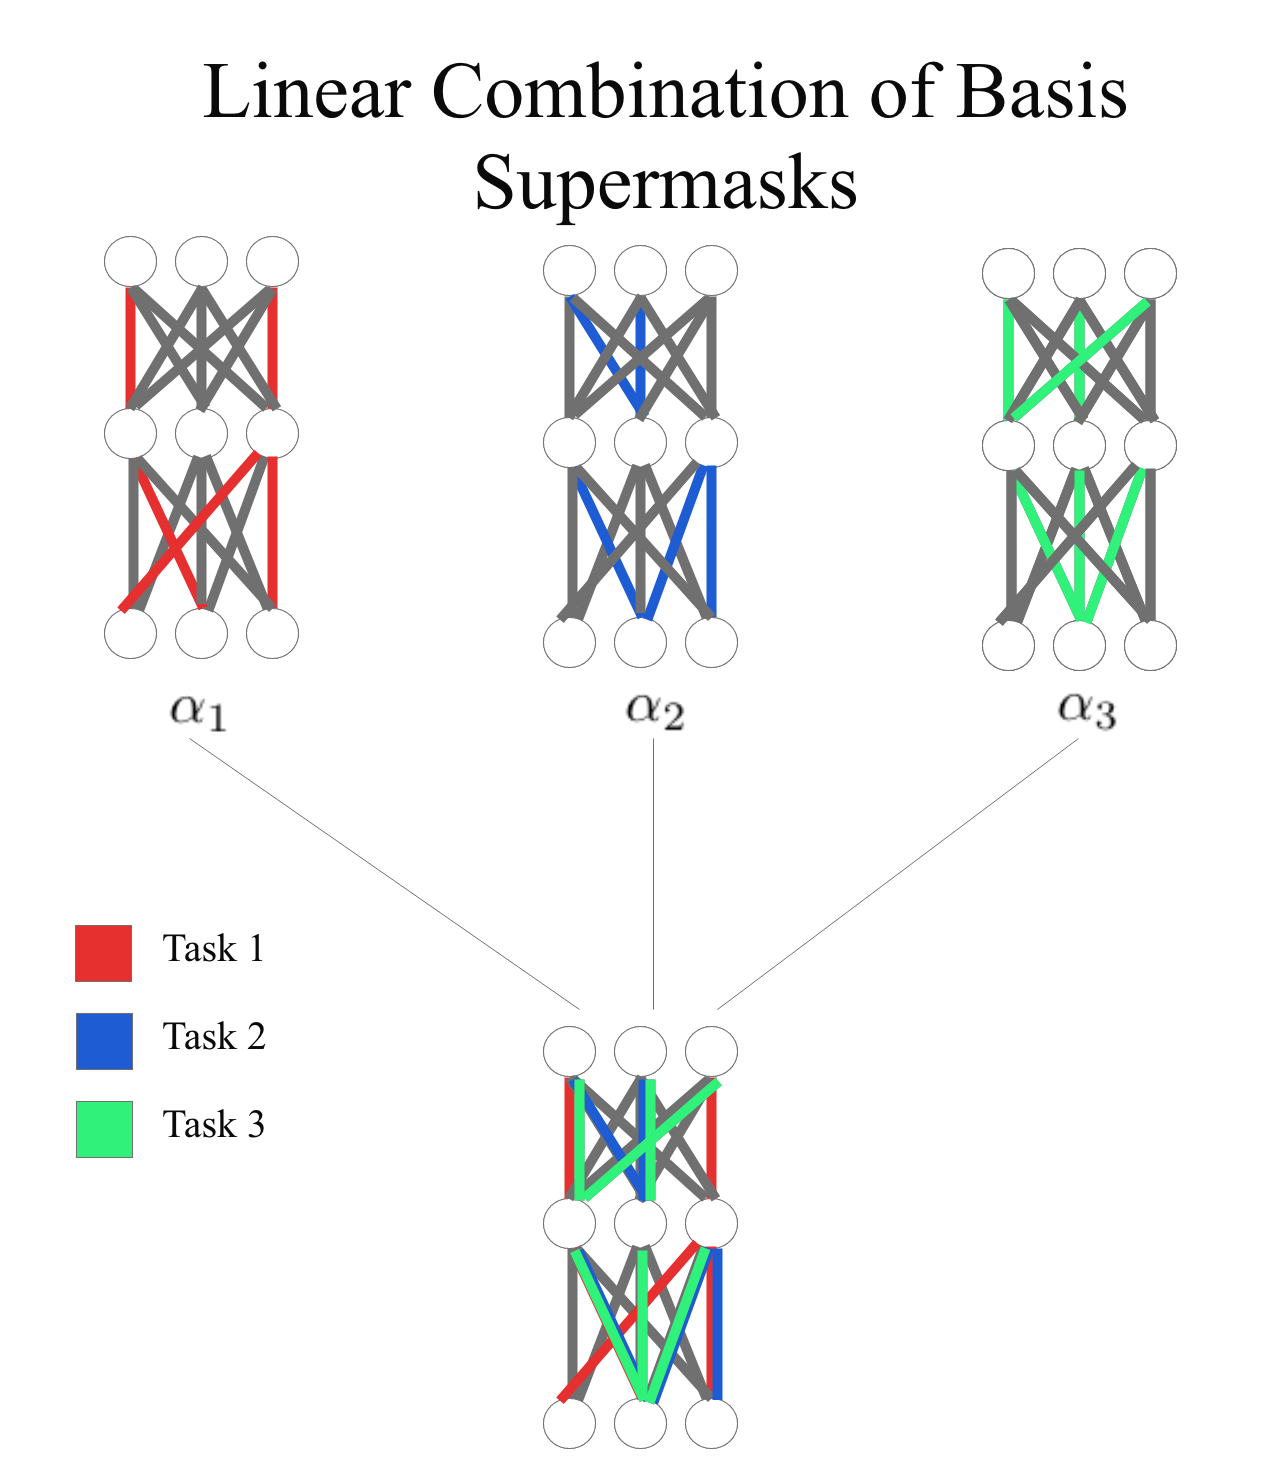
\includegraphics[width=5cm]{neural.png}
    %\caption{}
\end{figure}


An intuitive way to think about the algorithm is through neural network pathways. Inherently, supermasks either activate our deactivate neural network pathways to determine which weights are applied to a given task, according to weight importance. The core problem our team sought to explore was how to expand and apply methods in the space of continual learning to combat catastrophic forgetting. One algorithmic parameter that prior researchers have optimized is weight assignment. The SupSup approach proposed keeping static weights and instead identifying the most important pathways to "turn on" or "turn off". Our approach expands this method by selecting a randomly initialized set of weights and then combining these vector weights from learned tasks to create the following new masks for new and unseen tasks. This vector combination is nontrivial, and various researchers have proposed different ways of combining these vectors. 

We propose an approach rooted in linear algebra and deep learning--the basis vector approach. To combine these vectors, we calculate the sum of their products to create a new mask for unseen and unlearned tasks. 

As shown in the pseudocode attached:

\begin{lstlisting}[language=Python, caption=Linear Combination Approach Pseudocode]
class BasisMultitaskMaskConv(nn.Conv2d):

    def __init__(self, *args, **kwargs):
        super().__init__(*args, **kwargs)

        self.scores = nn.ParameterList(
            [
                nn.Parameter(module_util.mask_init(self))
                for _ in range(pargs.num_seed_tasks_learned)
            ]
        )
        for s in self.scores:
            s.requires_grad = False
        self.scores.requires_grad = False
        if pargs.train_weight_tasks == 0:
            self.weight.requires_grad = False

        if pargs.start_at_optimal:
            self.basis_alphas = nn.ParameterList(
                [
                    nn.Parameter(torch.eye(pargs.num_seed_tasks_learned)[i])
                    for i in range(pargs.num_seed_tasks_learned)
                ]
                +
                [
                    nn.Parameter(torch.ones(pargs.num_seed_tasks_learned)/pargs.num_seed_tasks_learned)
                    for _ in range(pargs.num_seed_tasks_learned, pargs.num_tasks)
                ]
            )
        else:
            self.basis_alphas = nn.ParameterList(
                [
                    nn.Parameter(torch.ones(pargs.num_seed_tasks_learned)/pargs.num_seed_tasks_learned)
                    for _ in range(pargs.num_tasks)
                ]
            )
        self.sparsity = pargs.sparsity

    def forward(self, x):
        if pargs.use_single_mask > -1:
            subnet = module_util.GetSubnet.apply(
                self.scores[pargs.use_single_mask].abs(), self.sparsity
            )
            w = self.weight * subnet
        elif self.task < pargs.num_seed_tasks_learned and not pargs.train_mask_alphas:
            subnet = module_util.GetSubnet.apply(
                self.scores[self.task].abs(), self.sparsity
            )
            w = self.weight * subnet
        else:
            subnet = module_util.GetSubnet.apply(
                self.scores[0].abs(), self.sparsity
            )
            task_alpha = self.basis_alphas[self.task]
            w = self.weight * subnet * task_alpha[0]
            for i in range(1, pargs.num_seed_tasks_learned):
                subnet = module_util.GetSubnet.apply(
                    self.scores[i].abs(), self.sparsity
                )
                w += self.weight * subnet * task_alpha[i]

        x = F.conv2d(
            x, w, self.bias, self.stride, self.padding, self.dilation, self.groups
        )
        return x
\end{lstlisting}



\subsection{Main Contributions}

\paragraph{Contribution 1}
Proposed algorithmic approach that aims to achieve higher efficiency by using linear combinations of weights (?)


\section{Experimental Evaluation}

\subsection{Data}
The dataset used for the baseline model is CIFAR100. The CIFAR-100 dataset contains a labeled subset 80 million tiny images.\footnote{See the dataset source here: \href{https://www.cs.toronto.edu/~kriz/cifar.html}{https://www.cs.toronto.edu/~kriz/cifar.html}}
 Based on the original approach of Wortsman et al. and Wen et al., we randomly split the CIFAR100 dataset into 20 [ ** validate this number ] random partitions. We applied this splitting methodology using NYU's Prince cluster, on NVIDIA GPUs. 

\subsection{Methodology}

\subsection{Results}

\subsection{Discussion}

\section{Conclusions}

\subsection{Caveats}

\subsection{Areas of Future Research}

\section{Lessons Learned}
\subsection{Broader Impact}

\section*{References}
\small
* note: clean this up later and cite properly

[1] McCloskey, Michael; Cohen, Neal J. (1989). Catastrophic Interference in Connectionist Networks: The Sequential Learning Problem. Psychology of Learning and Motivation. 24. pp. 109–165. doi:10.1016/S0079-7421(08)60536-8. ISBN 978-0-12-543324-2.

[2] Ratcliff, Roger (1990). "Connectionist models of recognition memory: Constraints imposed by learning and forgetting functions". Psychological Review. 97 (2): 285–308. doi:10.1037/0033-295x.97.2.285. PMID 2186426.

[3] French, Robert M. (1991). Using Semi-Distributed Representations to Overcome Catastrophic Forgetting in Connectionist Networks (PDF). Proceedings of the 13th Annual Cognitive Science Society Conference. New Jersey: Lawrence Erlbaum. pp. 173–178. CiteSeerX 10.1.1.1040.3564.

[4] Piggyback paper

[5] SupSup Paper 

[6] Continual learning via Neural pruning paper 

[7] Mallya and Lazebnik, 2018

[8] Ramanujan et all, (Paper on how they find the Supermasks): [https://arxiv.org/pdf/1911.13299.pdf]


\section*{Appendix}


\end{document}